\rhead{Multi-robot Coordination}


\chapter{Multi-robot Coordination}
\label{sec:multi_robot}

\begin{figure}[!h]
\centering
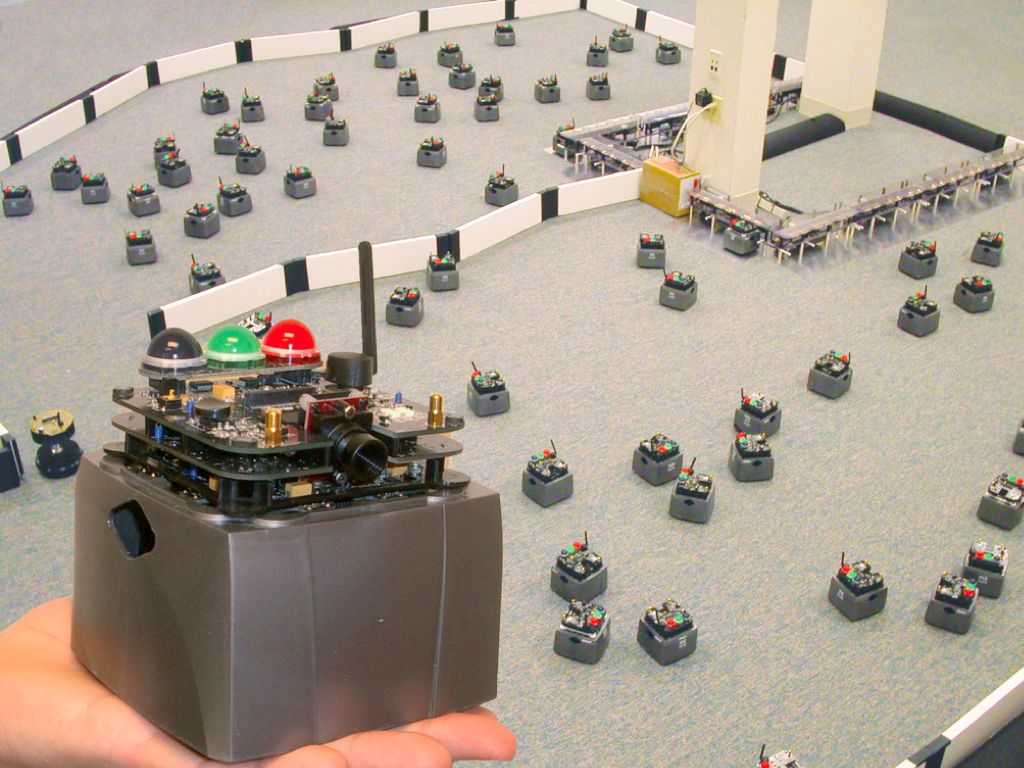
\includegraphics[width=1.0\columnwidth]{figures/10_teaser.jpg}
\end{figure}

\newpage

Given a team of Create robot platforms, develop a competitive multi-robot strategy and individual controllers

\section{Introduction}

Robot soccer challenge in a public space.

\begin{figure}[!h]
\centering
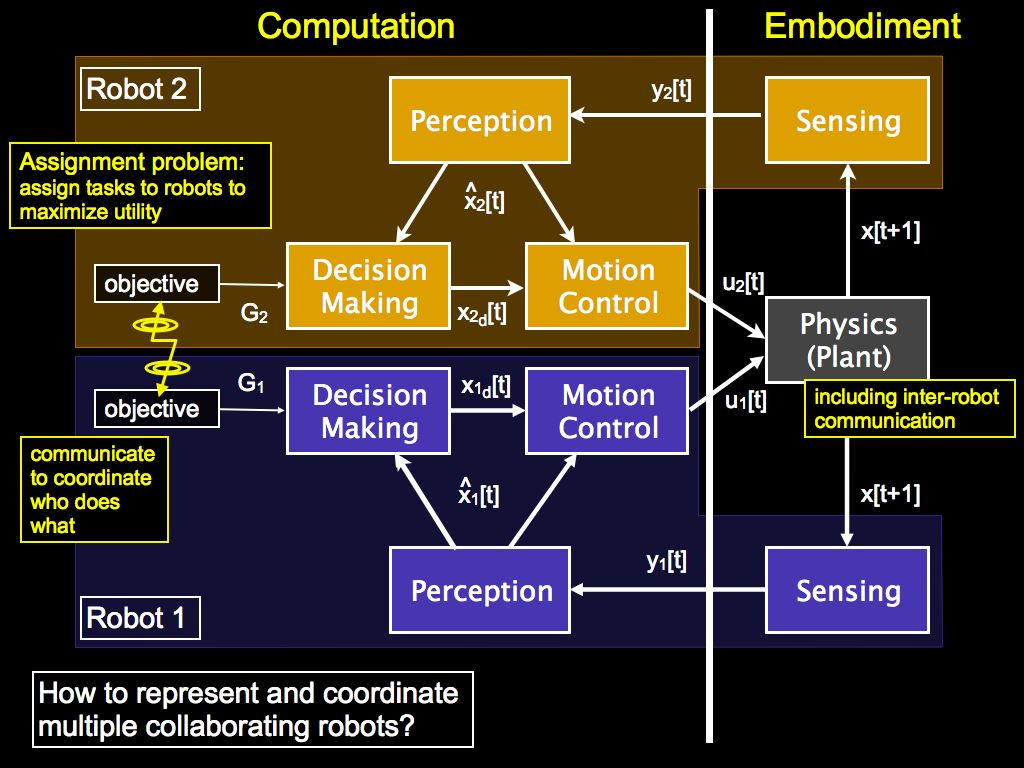
\includegraphics[width=0.8\columnwidth]{figures/10_control_loop.jpg}
\end{figure}

\begin{figure}
\centerline{
\mbox{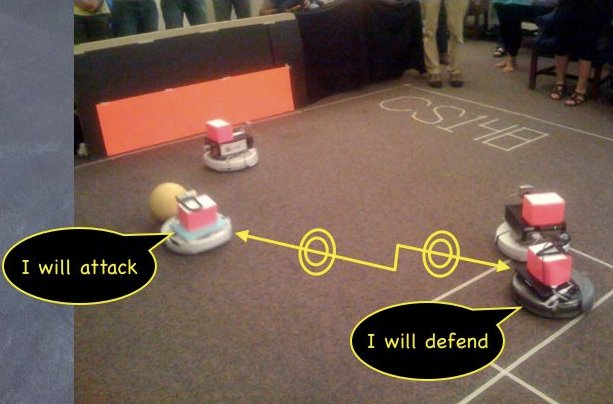
\includegraphics[width=3.00in]{figures/10_coordination1.jpg}}
\mbox{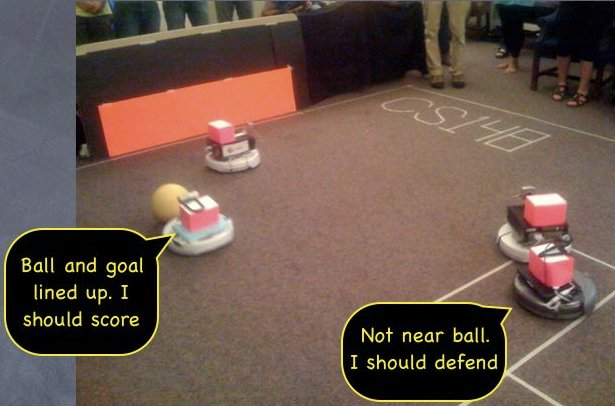
\includegraphics[width=3.00in]{figures/10_coordination2.jpg}}
}
\end{figure}

\section{Key Concepts}

\begin{figure}[!h]
\centering
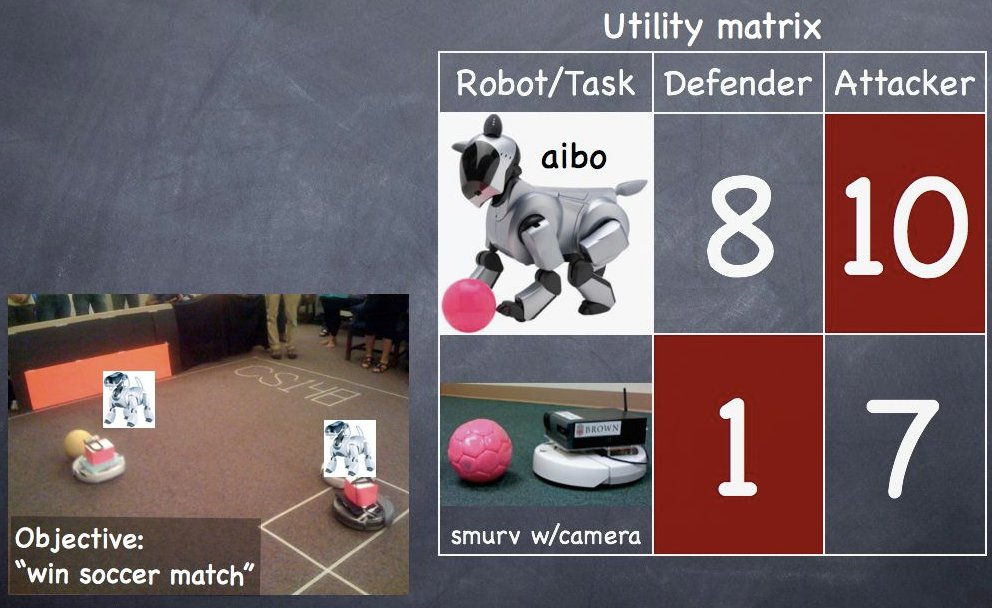
\includegraphics[width=0.8\columnwidth]{figures/10_soccer_example1.jpg}
\caption{Soccer Example: Greedy allocation?}
\end{figure}

\begin{figure}[!h]
\centering
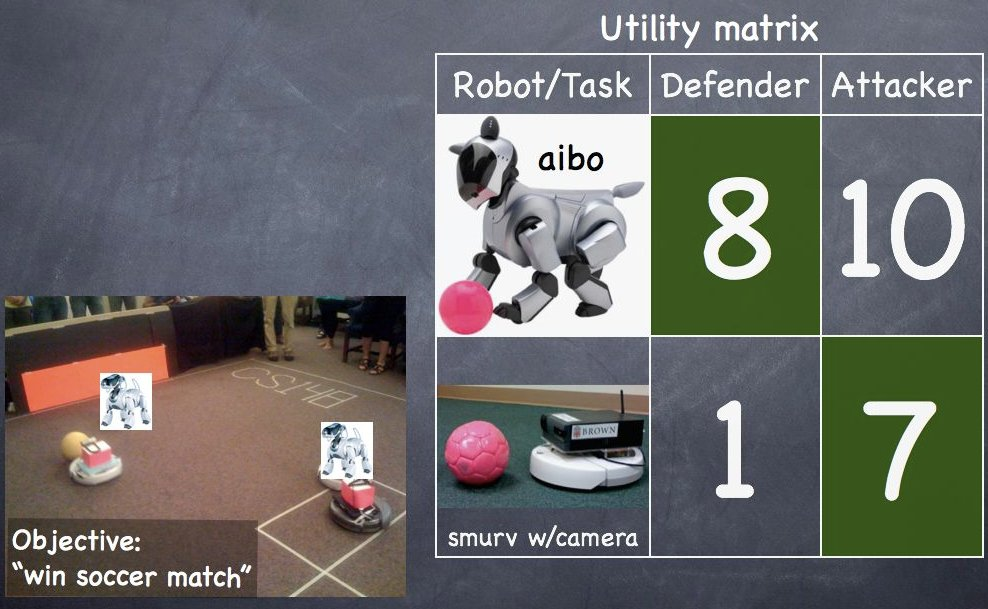
\includegraphics[width=0.8\columnwidth]{figures/10_soccer_example2.jpg}
\caption{Soccer Example: Optimal allocation}
\end{figure}

\begin{figure}[!h]
\centering
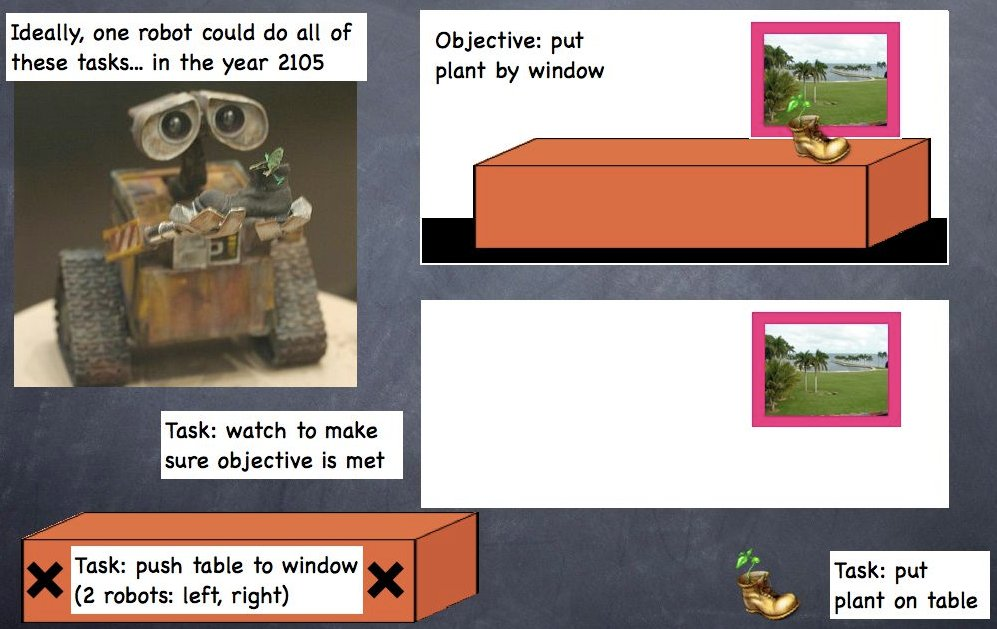
\includegraphics[width=0.8\columnwidth]{figures/10_directive_example.jpg}
\caption{``Directive" Example}
\end{figure}

\begin{figure}[!h]
\centering
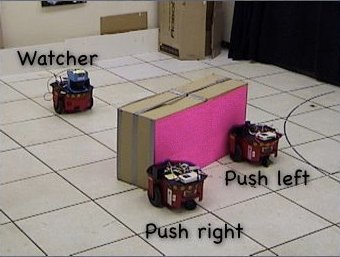
\includegraphics[width=0.5\columnwidth]{figures/10_box_example1.jpg}
\caption{Box pushing task setup}
\end{figure}

\begin{figure}[!h]
\centering
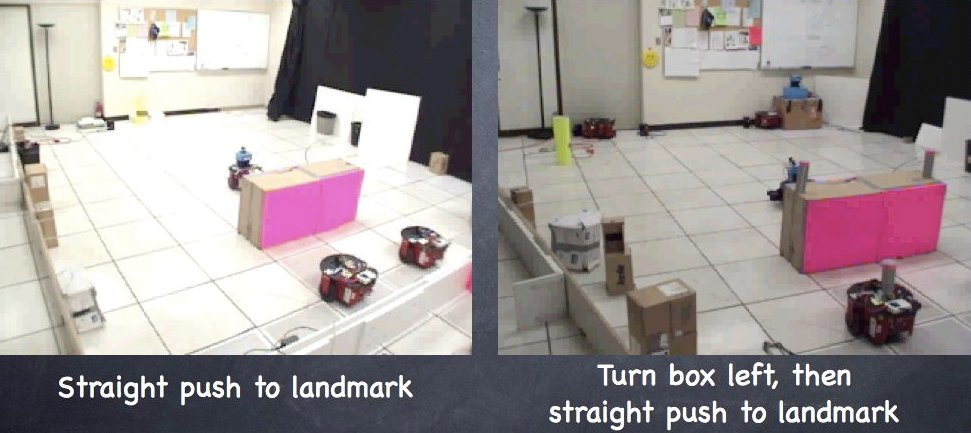
\includegraphics[width=1.0\columnwidth]{figures/10_box_example2.jpg}
\caption{Box pushing task approach}
\end{figure}

\begin{figure}[!h]
\centering
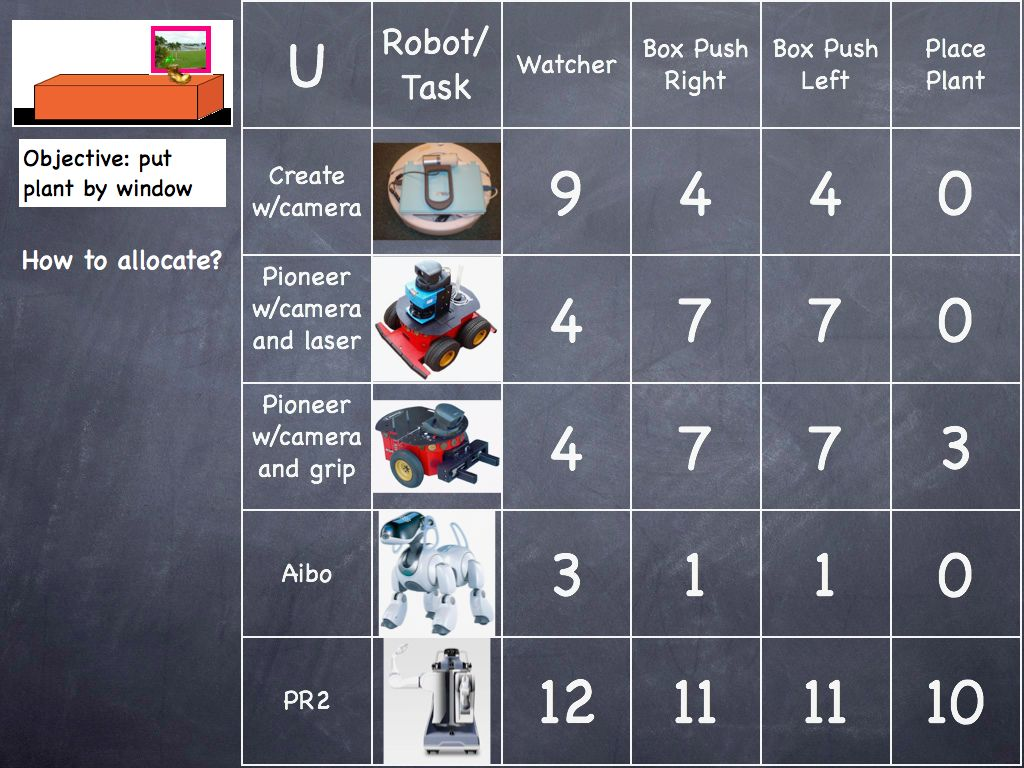
\includegraphics[width=0.8\columnwidth]{figures/10_plant.jpg}
\caption{Objective: put plant by window}
\end{figure}

\begin{figure}[!h]
\centering
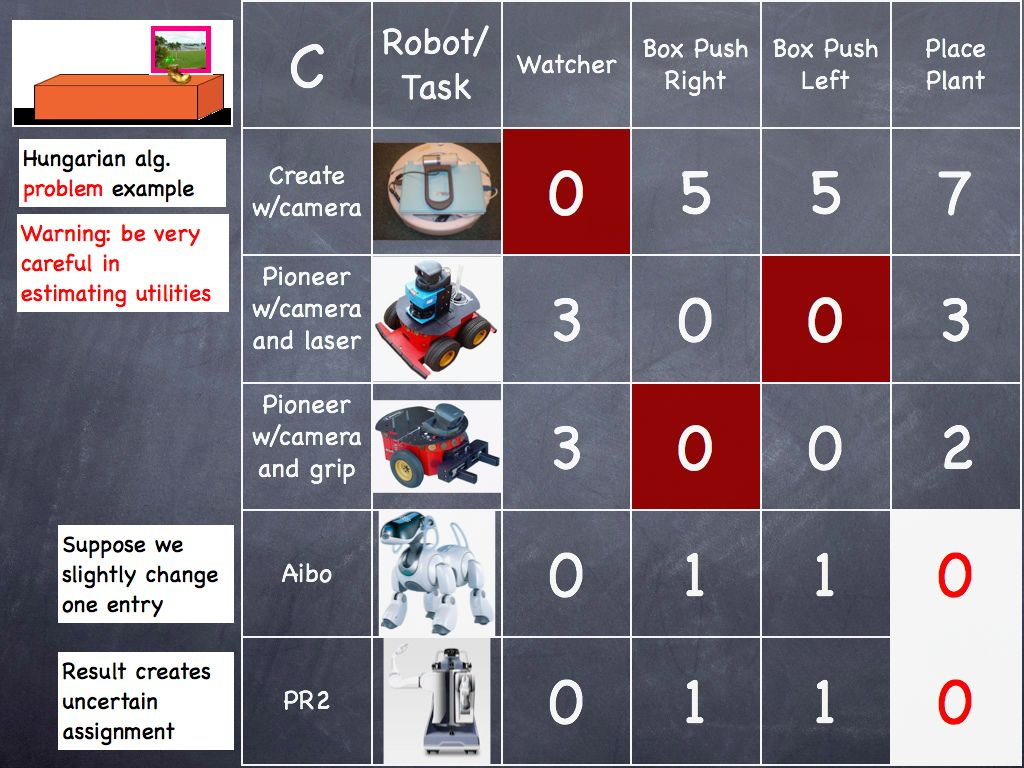
\includegraphics[width=0.8\columnwidth]{figures/10_hungarian.jpg}
\caption{Hungarian algorithm problem example}
\end{figure}

\section{Infrastructure}

\section{Instructions}

\section{Expected Outcomes and Reports}

\newpage
